This dissertation studies the information content of mandatory risk factor disclosures filed in annual reports by public firms in the United States.




\section{Hypothesis Development}\label{sec:supply_hypothesis}

The requirement to disclose risk factors is set forth in Item 503(c) of Regulation S-K:
\begin{quote}\singlespacing
	\textbf{\S 229.503 (Item 503) (c) Risk factors}. 
	Where appropriate, provide under the caption ``Risk Factors'' a discussion of the most significant factors that make the offering speculative or risky. 
	This discussion must be concise and organized logically. 
	Do not present risks that could apply to any issuer or any offering. 
	Explain how the risk affects the issuer or the securities being offered. 
	Set forth each risk factor under a subcaption that adequately describes the risk.
\end{quote}



\section{Sample Construction and Data Collection}\label{sec:sample}

Risk Factor disclosures have been required in annual and quarterly disclosures under Item 1A since the SEC regulation took effect in 2005.


\begin{thesistable}{Summary Stats}{\ref{tab:summarystats}}
	\label{tab:summarystats}
	
	Table \ref{tab:summarystats} reports the summary statistics for the variables used in the regressions as defined in Appendix \ref{App:vardef}.
	
	\startdata
	\begin{tabular}{l*{1}{cccccccc}} \toprule
	                                   &  Mean   & Std. Dev &  Min  & 25\%  & 50\%  &  75\%  &  Max   &   N    \\ \midrule
	$ Log(Assets)_{t} $                &  6.70   &   2.01   & 2.12  & 5.34  & 6.74  &  8.05  & 11.56  & 26,547 \\
	$ Log(Market\ Equity)_{t} $        &  6.33   &   1.96   & 1.84  & 4.99  & 6.35  &  7.70  & 10.56  & 26,537 \\
	$ Book-to-Market_{t} $             &  0.73   &   0.90   & -0.71 & 0.31  & 0.58  &  0.96  &  4.60  & 26,518 \\
	$ Sales / AT_{t} $                 &  0.90   &   0.85   & 0.00  & 0.26  & 0.70  &  1.27  &  4.04  & 26,536 \\
	$ Beta_{t-1} $                     &  1.04   &   0.54   & -0.10 & 0.69  & 1.05  &  1.40  &  2.31  & 26,547 \\ \midrule \addlinespace 
    \multicolumn{9}{c}{\normalsize Indicator and Negative Outome Variables}                                    \\ \midrule
	$ Negative\ NI_{t+1} $             &  0.31   &   0.46   &   0   &   0   &   0   &   1    &   1    & 22,026 \\
	$ Sec.\ Litigation_{t-1} $         &  0.02   &   0.14   &   0   &   0   &   0   &   0    &   1    & 26,546 \\
	$ Lawsuit\ Intensity_{t-1} $       &  0.19   &   0.44   &   0   &   0   &   0   &   0    &  2.08  & 26,547 \\
	$ RF\ Comment_{t-1} $              &  0.07   &   0.25   &   0   &   0   &   0   &   0    &   1    & 26,224 \\
	$ Comment\ (Any)_{t-1} $           &  0.53   &   0.50   &   0   &   0   &   1   &   1    &   1    & 26,223 \\ \midrule \addlinespace
    \multicolumn{9}{c}{\normalsize Textual Variables}                                                          \\ \midrule
	$ \#\ Risk\ Factors_{t} $          &  29.52  &  14.05   &   6   &  19   &  27   &   37   &   69   & 26,547 \\
	$ \#\ New\ RF_{t} $                &  3.67   &   5.03   &   0   &   1   &   2   &   5    &   25   & 26,547 \\
	$ \#\ Dropped\ RF_{t} $            &  2.45   &   3.73   &   0   &   0   &   1   &   3    &   21   & 26,547 \\
    $ \Delta \#\ RF_{t} $              &   1.22  &   4.56   & -11   &   0   &   1   &   2    &   18   & 26,547 \\ \bottomrule
\end{tabular}
\end{thesistable}

The average firm in my sample has 29.5 risk factors, and adds 3.7 new risks and removes 2.5 obsolete risks per year.
I find that younger firms (below the median firm age of 13 years) disclose 34.4 risk factors on average, and identify 4.4 new factors per year and remove 3.2 factors.
Older firms (above median age) disclose significantly fewer risk factors, only 25.8, and identify new factors and remove old factors at significantly lower rates as well (3.4 and 2.2, respectively).
This potentially suggests life cycle effects in risk factor disclosures, with older, more established, and less volatile firms disclosing fewer risks and experiencing less risk `turnover.'
However, when looking at the change in word count of the risk factors between these two groups, there is no significant difference.%
\footnote{The change in word counts are 135.5 and 136.4 for young and old firms respectively (t-stat = -0.16). The t-stat for difference in new, dropped, and total risk factors are all significant at \textless 0.001 level.}
This suggests that the time series evolution of risk factors may capture some underlying economic differences that a word count approach does not.
A graphical depiction of this trend is presented in Figure \ref{fig:rf_ageseries}.


\begin{figure}[ht!]
	\caption{New and Removed Risk Factors Over Firm Age}
	\label{fig:rf_ageseries}
	
	Figure \ref{fig:rf_ageseries} plots the average number of new and removed risk factors over the age of the firm.
	The datapoints represent averages over five year periods.
	The sample comprises firm-years with a non-missing risk factor section in the previous year.
	
	\skipline
	\centering
	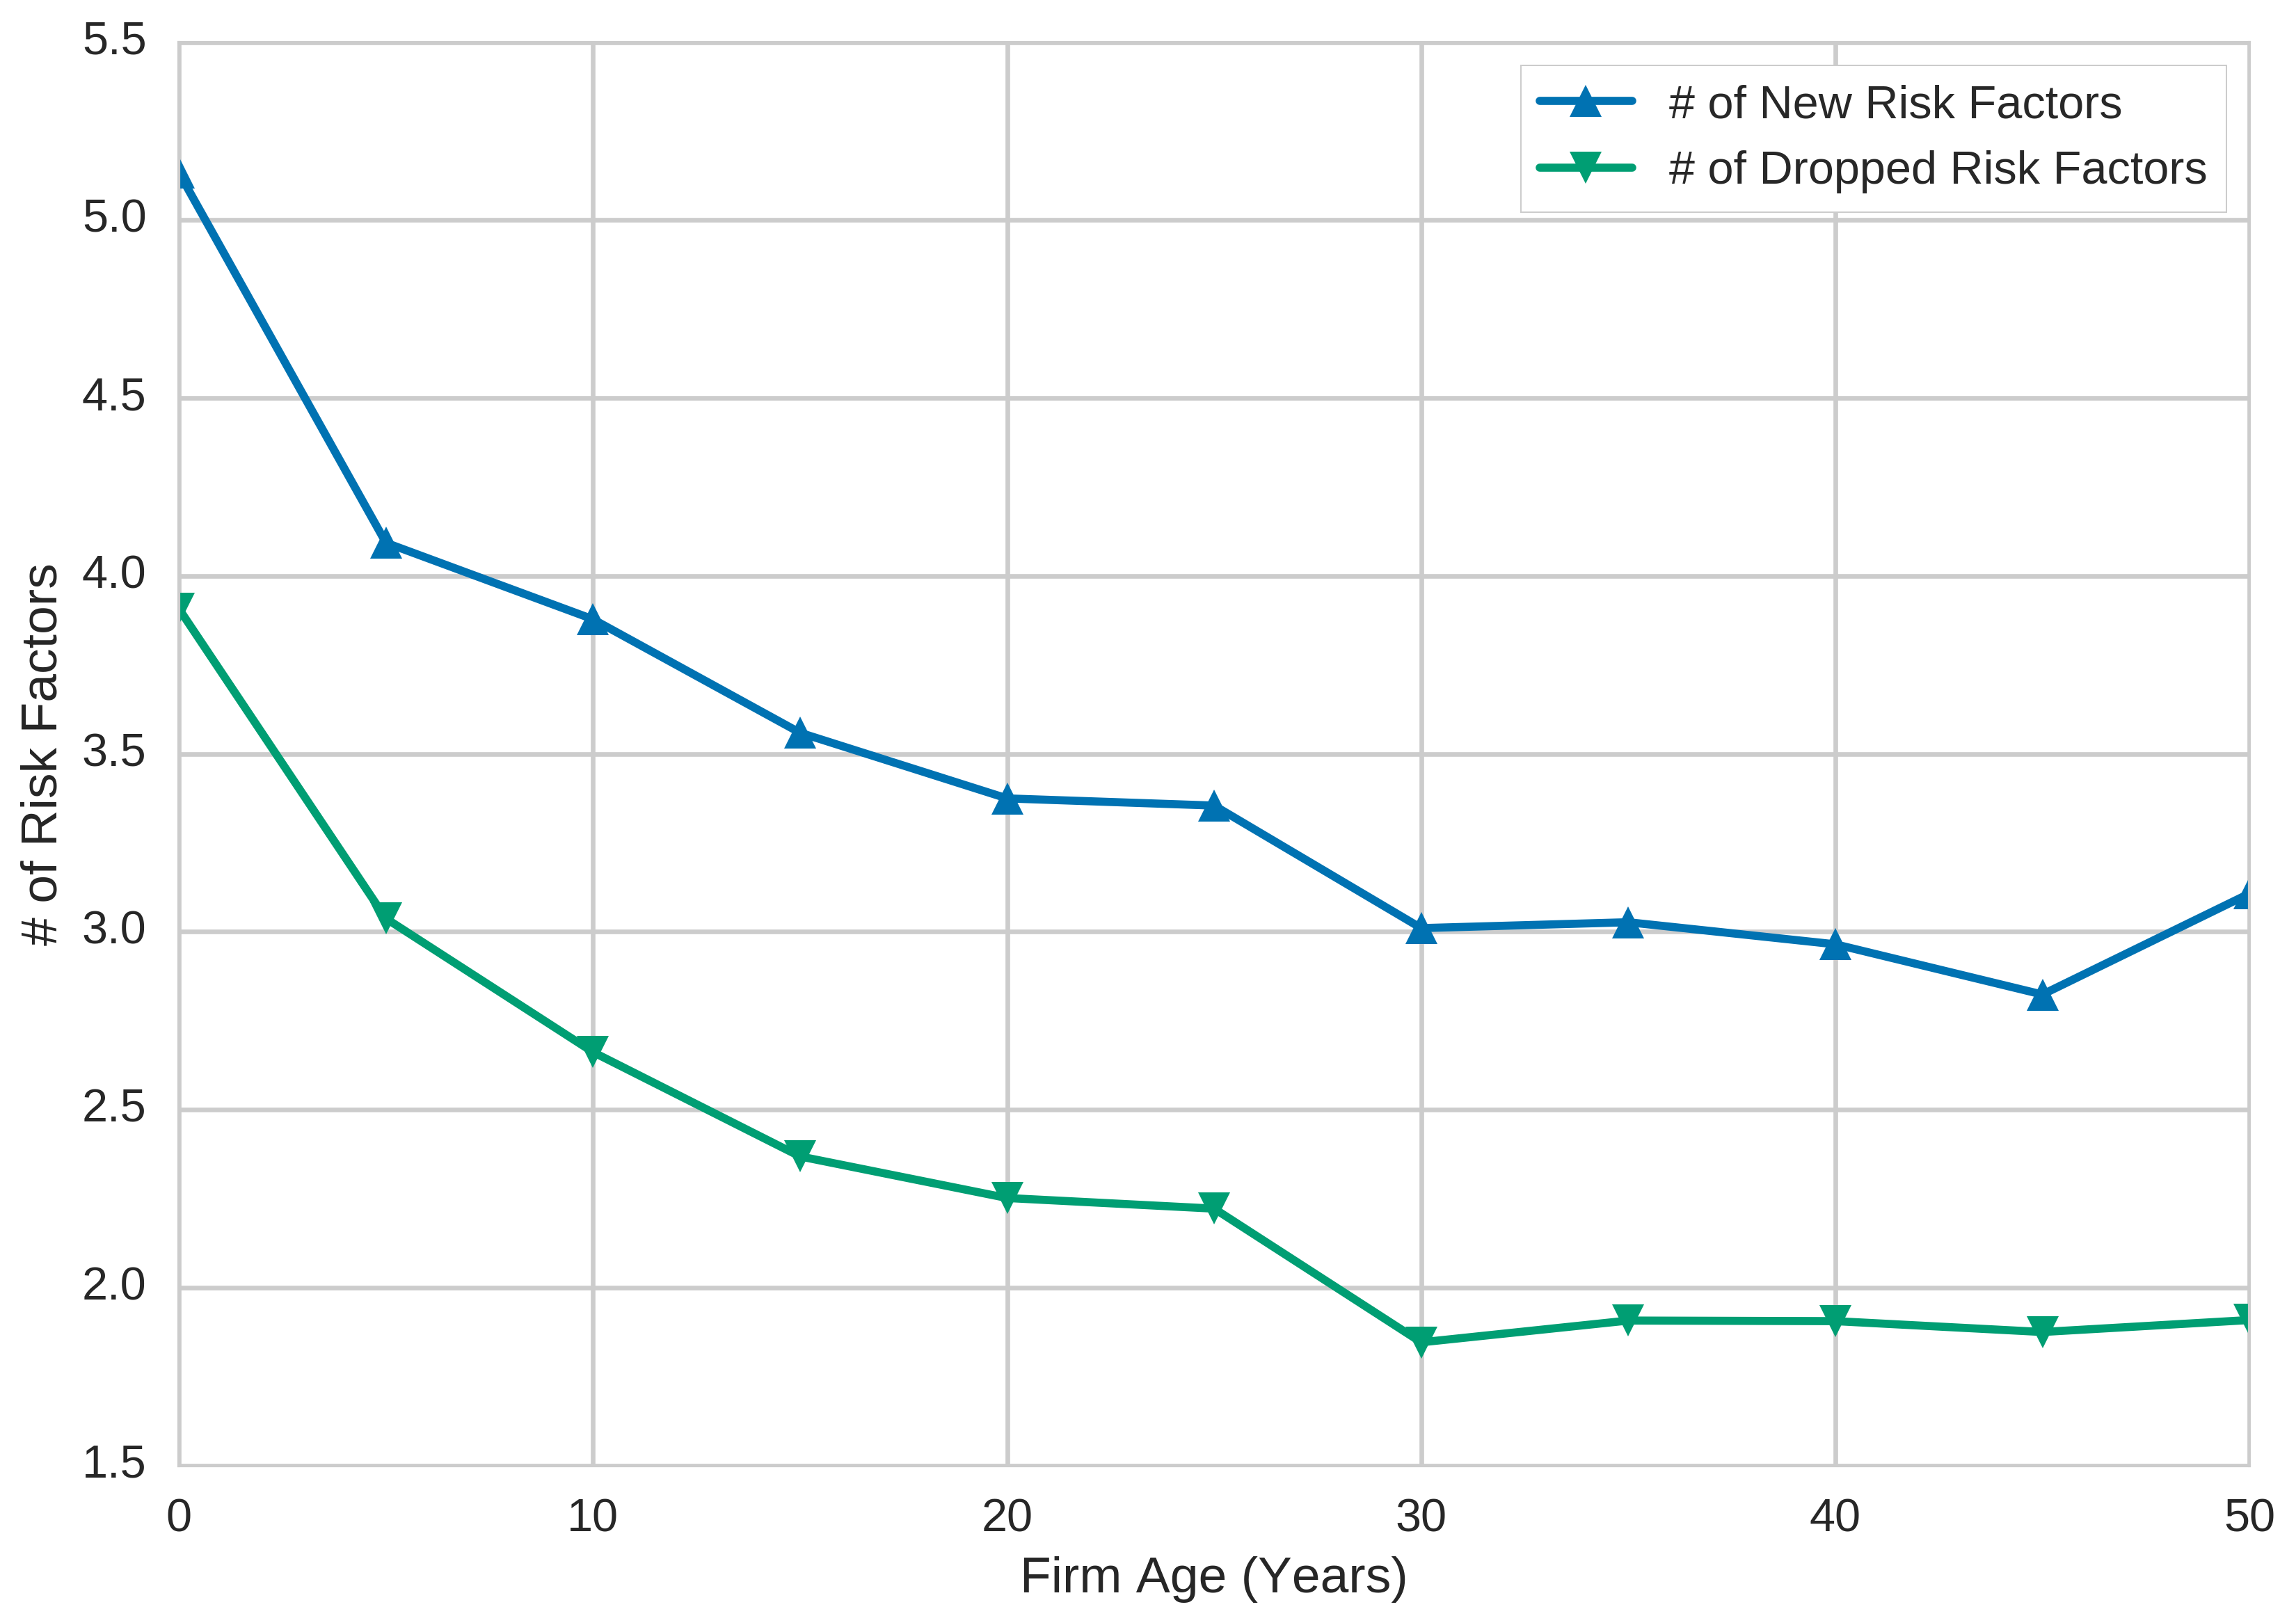
\includegraphics[scale=.5]{figures/add-drop_over_age.png}
\end{figure}




\section{Results}\label{sec:supply_result}

QED.




\subsection{Alternative Specifications}\label{sec:supply_robustness}

QED again.

